\section{Régulateur PID}

\subsection{Introduction}
Afin de réguler les variations en sortie $PV$, on utilise un régulateur PID, qui reprend la valeur de $PV$ pour la soustraire à la consigne $SP$ donnant donc l'erreur $E = SP - PV$ à corriger sur $MV$.\\
Pour rappel, un régulateur PID est composé de trois termes:
\begin{itemize}
    \item Le terme proportionnel $P$ qui est proportionnel à l'erreur $E$ et vise une erreur statique nulle.
    \item Le terme intégral $I$ qui est proportionnel à la somme des erreurs passées et donc accumule l'erreur.
    \item Le terme dérivé $D$ qui est proportionnel à la dérivée de l'erreur et vise à corriger anticipativement l'erreur future.
\end{itemize}
La sortie du régulateur est alors donnée par :
\begin{equation}
    MV = K_C \, \left( 1 + \frac{1}{T_I s} + \frac{T_D s}{\alpha T_D s + 1}\right) \, E
\end{equation}

Dans le cadre du laboratoire, le régulateur utilise également le \textbf{Reset de l'Action Intégrale} et la \textbf{Saturation de l'Action Intégrale} venant adapter l'action intégrale en fonction de, respectivement, la valeur de $MV$ en mode manuel, et la saturation de $MV$ atteignant les limites $MV_{MAX}$ / $MV_{MIN}$.
\begin{center}
    $MV_I = MV_{Man} - MV_P - MV_D - MV_{FF}$\\[4pt]
    et\\[4pt]
    $MV_I = MV_{MAX} - MV_P - MV_D - MV_{FF}$
\end{center}

\subsection{Optimisation par la méthode IMC}
Il est important de choisir les paramètres $K_C$, $T_I$ et $T_D$ de façon à implémenter le bon régulateur pour notre processus.
Une façon d'obtenir ces paramètres optimaux est de réaliser un step sur $MV$ et d'observer la dynamique du Processus.
Le modèle trouvé va nous permettre de calculer ces valeurs via des tables.\\
On utilisera la ligne I du tableau présent dans le cours, correspondant à un modèle du second ordre avec délai ($\tau_3 = 0$).
\begin{align*}
    K_C &= \frac{1}{K_P} \, \frac{T_{1p} + T_{2p}}{T_{CLP} + \theta}\\[4pt]
    T_I &= T_{1p} + T_{2p}\\[4pt]
    T_D &= \frac{T_{1p} \, T_{2p}}{T_{1p} + T_{2p}}
\end{align*}
Il est bon de noter que nous aurions pu utiliser la ligne G du tableau (premier ordre avec délai) totalement équivalente étant donné que notre Processus est du premier ordre ($T_{2p} \approx 0$).
\begin{align*}
    K_C &= \frac{1}{K_P} \, \frac{T_{1p}}{T_{CLP} + \theta}\\[4pt]
    T_I &= T_{1p}\\[4pt]
    T_D &= 0
\end{align*}
La constante de temps en boucle fermée $T_{CLP}$ est un certain ratio de la première constante de temps du processus $T_{1p}$ définit par $T_{CLP} = \gamma \, T_{1p}$. L'influence de $\gamma$ sera discuté en simulation de boucle fermée par après.

\subsection{Réponse indicielle du régulateur PID}

Nous allons maintenant analyser la réponse du régulateur lorsqu'on applique une erreur $E$ constante à son entrée.
\begin{figure}[H]
    \centering
    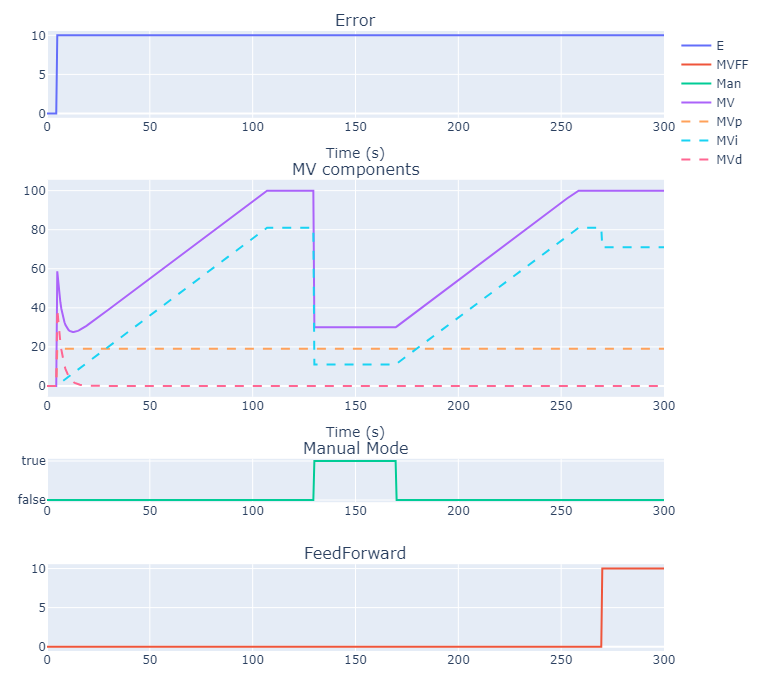
\includegraphics[width=0.9\textwidth]{../Plots/PID/PID_Response_error_step.png}
    \caption{Réponse indicielle du PID à un step sur E}
    \label{fig:Step_Response_PID}
\end{figure}

